\documentclass[11pt,letterpaper]{article}
\usepackage[utf8]{inputenc}
\usepackage[T1]{fontenc}
\usepackage[provide=*,spanish]{babel}
\usepackage[letterpaper,margin=1.8cm,top=1.9cm,bottom=1.8cm]{geometry}
\usepackage{lmodern,microtype,amsmath,amssymb,booktabs,graphicx,fancyhdr,array,listings,tabularx,tikz,titlesec}
\usepackage[table]{xcolor}
\usepackage[hidelinks]{hyperref}
\definecolor{Tinta}{HTML}{152C45}
\definecolor{Azul}{HTML}{164B70}
\definecolor{Oro}{HTML}{B9955E}
\definecolor{Fondo}{HTML}{F1F5F8}
\definecolor{Gris}{HTML}{556475}
\definecolor{Linea}{HTML}{D3DDE6}
\color{Tinta}
\setlength{\parindent}{0pt}
\setlength{\parskip}{7pt}
\setlength{\emergencystretch}{2em}
\setlength{\headheight}{21pt}
\setlength{\headsep}{15pt}
\pagestyle{fancy}\fancyhf{}
\fancyhead[L]{\sffamily\scriptsize\color{Gris}FUNDAMENTOS DE BASES DE DATOS}
\fancyhead[R]{\sffamily\scriptsize\color{Gris}TAREA 04 / ÁLGEBRA RELACIONAL}
\fancyfoot[L]{\sffamily\scriptsize\color{Gris}UNAM · Facultad de Ciencias}
\fancyfoot[C]{\sffamily\small\thepage}
\fancyfoot[R]{\sffamily\scriptsize\color{Gris}Equipo ÑIPGG}
\renewcommand{\headrule}{\hbox to\headwidth{\color{Linea}\leaders\hrule height .4pt\hfill}}
\renewcommand{\footrulewidth}{0pt}
\titleformat{\section}{\sffamily\Large\bfseries\color{Azul}}{}{0pt}{}[\vspace{2pt}{\color{Oro}\titlerule[.8pt]}]
\titleformat{\subsection}{\sffamily\large\bfseries\color{Azul}}{}{0pt}{}
\titlespacing*{\section}{0pt}{5pt}{12pt}
\titlespacing*{\subsection}{0pt}{13pt}{7pt}
\newcommand{\seccion}[1]{\phantomsection\section*{#1}\addcontentsline{toc}{section}{#1}}
\lstset{basicstyle=\ttfamily\scriptsize\color{Tinta},breaklines=true,columns=fullflexible,frame=single,rulecolor=\color{Linea},backgroundcolor=\color{Fondo},framesep=6pt,xleftmargin=6pt,xrightmargin=6pt,aboveskip=9pt,belowskip=10pt,showstringspaces=false}
\newcommand{\caprel}[3]{\begin{center}\includegraphics[width=\linewidth,height=#2cm,keepaspectratio]{\RutaMiguel/evidencias/#1}\par\vspace{4pt}{\sffamily\footnotesize\color{Gris}#3}\end{center}}
\hypersetup{pdftitle={Tarea 04 - Álgebra relacional},pdfauthor={Equipo ÑIPGG},pdfsubject={Fundamentos de Bases de Datos, semestre 2027-I}}

\usepackage{longtable}
\usetikzlibrary{arrows.meta,positioning}
\tikzset{operador/.style={draw=Linea,fill=Fondo,rounded corners=3pt,align=center,font=\sffamily\small,text=Tinta,inner sep=7pt},flujo/.style={-{Latex[length=2mm]},draw=Azul,thick}}
\newcommand{\nulo}{\texttt{null}}

\newcommand{\leftouterjoin}{\mathbin{\ooalign{$\bowtie$\cr\hidewidth\raise.15ex\hbox{\scalebox{1.15}[1]{$\lbrack$}}\kern.7em\hidewidth\cr}}}
\newcommand{\rightouterjoin}{\mathbin{\ooalign{$\bowtie$\cr\hidewidth\kern.7em\raise.15ex\hbox{\scalebox{1.15}[1]{$\rbrack$}}\hidewidth\cr}}}
\lstset{literate={⟕}{{$\leftouterjoin$}}1 {⟖}{{$\rightouterjoin$}}1}

\newcommand{\RutaMiguel}{..}
\begin{document}
\hypersetup{pageanchor=false}
\begin{titlepage}
\thispagestyle{empty}
\begin{tikzpicture}[remember picture,overlay]
\fill[Tinta] (current page.north west) rectangle ([yshift=-9.4cm]current page.north east);
\fill[Oro] ([yshift=-9.4cm]current page.north west) rectangle ([yshift=-9.52cm]current page.north east);
\node[anchor=north east,text=white,opacity=.07,font=\sffamily\bfseries\fontsize{150}{150}\selectfont] at ([xshift=-.8cm,yshift=-2.4cm]current page.north east) {04};
\end{tikzpicture}
{\color{white}\sffamily
{\large Universidad Nacional Autónoma de México\par}
\vspace{2pt}{\normalsize Facultad de Ciencias\par}
\vspace{.85cm}
{\small\bfseries\color{Oro}FUNDAMENTOS DE BASES DE DATOS\par}
\vspace{.35cm}
{\fontsize{38}{42}\selectfont\bfseries Tarea 04\par}
\vspace{.2cm}
{\fontsize{25}{30}\selectfont Álgebra relacional\par}
\vspace{.45cm}
{\small Cardinalidad · Consultas · Mantenimiento de datos\par}}
\vspace{1.9cm}
{\sffamily\color{Azul}\Large\bfseries Equipo ÑIPGG\par}
\vspace{.35cm}
{\sffamily\small
\renewcommand{\arraystretch}{1.65}
\begin{tabularx}{\linewidth}{@{}Xr@{}}
\toprule
\textbf{Integrante} & \textbf{Número de cuenta}\\\midrule
Omar Alejandro Juárez Larrondo & 322245244\\
Yahir León Bautista & 322176542\\
Diego Hernández Gómez & 321069942\\
Miguel Ángel Jiménez Ramírez & 119000887\\
Ana Lilia Carballido Camacateco & 315314601\\
\bottomrule
\end{tabularx}\par}
\vfill
{\sffamily\small
\begin{tabularx}{\linewidth}{@{}Xr@{}}
\textcolor{Gris}{PROFESOR} & \textcolor{Gris}{SEMESTRE}\\[3pt]
Gerardo Avilés Rosas & 2027-I\\[12pt]
\textcolor{Gris}{FECHA DE ENTREGA} &\\[3pt]
30 de octubre de 2026 &\\
\end{tabularx}\par}
\vspace{.35cm}{\color{Oro}\rule{\linewidth}{.7pt}}
\end{titlepage}
\hypersetup{pageanchor=true}
\setcounter{page}{1}

\tableofcontents
\vspace{1cm}
\textbf{Contenido del módulo 03}\par
Miguel Ángel Jiménez Ramírez: cardinalidades C03 y C04, consultas 2.b y 2.f, y mantenimiento e.

Cada consulta y operación parte del dataset original. Las expresiones ejecutables y las evidencias acompañan este documento.
\clearpage
\seccion{1. Cardinalidad de las consultas}
Las relaciones iniciales son:\par
$R(A,B)=\{(1,x),(2,y),(2,z),(3,x),(9,a)\}$\par
$S(B,C,D)=\{(x,0,3),(y,2,1),(y,3,3),(w,3,0),(y,4,2)\}$.

Se usa semántica de conjuntos. C03 y C04 son juntas externas naturales: la coincidencia se establece por el atributo compartido $B$, que aparece una sola vez. La junta interna $R\bowtie S$ tiene cinco tuplas: dos para $B=x$ y tres para $B=y$. Los valores \nulo{} representan atributos faltantes.

\subsection*{C03. Junta externa izquierda $R\leftouterjoin S$}
Se conservan todas las tuplas de $R$. Las tuplas $(2,z)$ y $(9,a)$ no tienen pareja en $S$; se completan con \nulo{} en $C$ y $D$.
\[
R\leftouterjoin S=(R\bowtie S)\cup\{(2,z,\texttt{null},\texttt{null}),(9,a,\texttt{null},\texttt{null})\}.
\]
\begin{center}\begin{tabular}{cccc}\toprule\rowcolor{Fondo}
$A$ & $B$ & $C$ & $D$\\\midrule
1 & x & 0 & 3\\
2 & y & 2 & 1\\
2 & y & 3 & 3\\
2 & y & 4 & 2\\
2 & z & \nulo & \nulo\\
3 & x & 0 & 3\\
9 & a & \nulo & \nulo\\\bottomrule
\end{tabular}\end{center}
\textbf{Cardinalidad: 7 tuplas} ($5$ coincidencias y $2$ tuplas de $R$ sin pareja). La tupla $(2,y)$ se combina con tres tuplas distintas de $S$; sus valores de $C$ o $D$ difieren, por lo que no se generan duplicados.

\subsection*{C04. Junta externa derecha $R\rightouterjoin S$}
Se conservan todas las tuplas de $S$. La tupla $(w,3,0)$ no tiene pareja en $R$; se completa con \nulo{} en $A$.
\[
R\rightouterjoin S=(R\bowtie S)\cup\{(\texttt{null},w,3,0)\}.
\]
\begin{center}\begin{tabular}{cccc}\toprule\rowcolor{Fondo}
$A$ & $B$ & $C$ & $D$\\\midrule
1 & x & 0 & 3\\
3 & x & 0 & 3\\
2 & y & 2 & 1\\
2 & y & 3 & 3\\
\nulo & w & 3 & 0\\
2 & y & 4 & 2\\\bottomrule
\end{tabular}\end{center}
\textbf{Cardinalidad: 6 tuplas} ($5$ coincidencias y $1$ tupla de $S$ sin pareja). Las tuplas $(2,z)$ y $(9,a)$ de $R$ se excluyen. No hay duplicados.

\clearpage
\section*{1. Evidencias de cardinalidad en Relax}
\textbf{C03: expresión y comprobación}
\lstinputlisting{\RutaMiguel/cardinalidad_c03.relax}
\begin{center}
\begin{minipage}{.60\linewidth}\caprel{cardinalidad_c03_arbol.png}{4.4}{Árbol de la junta externa izquierda.}\end{minipage}\hfill
\begin{minipage}{.33\linewidth}\caprel{cardinalidad_c03_resultado.png}{4.8}{Resultado: 7 tuplas.}\end{minipage}
\end{center}
\textbf{C04: expresión y comprobación}
\lstinputlisting[firstline=15]{\RutaMiguel/cardinalidad_c04.relax}
\begin{center}
\begin{minipage}{.60\linewidth}\caprel{cardinalidad_c04_arbol.png}{4.4}{Árbol de la junta externa derecha.}\end{minipage}\hfill
\begin{minipage}{.33\linewidth}\caprel{cardinalidad_c04_resultado.png}{4.8}{Resultado: 6 tuplas.}\end{minipage}
\end{center}

\clearpage
\seccion{2.b. Productos de Technology sin órdenes}
Se buscan productos de la categoría \texttt{Technology} con precio estrictamente mayor que \$400 y menor que \$850, cuyo identificador no figure en ninguna orden. Se conservan los cuatro atributos del producto; los encabezados se renombran para facilitar su lectura.

\textbf{Expresión en álgebra relacional}
\begin{align*}
T &\leftarrow \sigma_{category='Technology'\,\land\,price>400\,\land\,price<850}(products)\\
P &\leftarrow \pi_{productid}(orders)\\
N &\leftarrow T-(T\bowtie P)\\
Resultado &\leftarrow \pi_{\substack{productid\to id,\ category\to categoria,\\subcategory\to tipo,\ price\to precio}}(N).
\end{align*}
La junta natural usa \texttt{productid}. Como $P$ solo contiene ese atributo, $T\bowtie P$ conserva el esquema de $T$ y la diferencia está bien definida. La proyección final cambia únicamente los nombres de las columnas.

\textbf{Expresión ejecutada en Relax}
\lstinputlisting{\RutaMiguel/consulta_b.relax}
\textbf{Resultado: 2 productos.} Hay 28 candidatos en el intervalo: 26 tienen al menos una orden y 2 no aparecen en ninguna. El resultado no es vacío.
\begin{center}\small\begin{tabular}{lllr}\toprule\rowcolor{Fondo}
id & categoria & tipo & precio\\\midrule
TEC-PH-10004080 & Technology & Phones & 487.98\\
TEC-MA-10004086 & Technology & Machines & 659.98\\\bottomrule
\end{tabular}\end{center}
\caprel{consulta_b_resultado.png}{7.6}{Resultado de la consulta 2.b en Relax, con las cuatro columnas.}

\clearpage
\section*{2.b. Árbol lógico de la consulta}
El árbol representa los operadores de la expresión ejecutable. Se lee de abajo hacia arriba; las etiquetas indican las cardinalidades comprobadas con el dataset original.
\begin{center}
\begin{tikzpicture}
\node[operador,text width=10cm] (out) at (0,0) {Proyección y renombrado\\$productid\to id$, $category\to categoria$,\\$subcategory\to tipo$, $price\to precio$\\\textbf{2 tuplas}};
\node[operador] (diff) at (0,-2.5) {Diferencia $T-(T\bowtie P)$\\\textbf{2 tuplas}};
\node[operador,text width=5cm] (t1) at (-3.7,-5) {$\sigma_{\substack{category='Technology'\\\land\,400<price<850}}$\\\textbf{28 tuplas}};
\node[operador] (join) at (3.7,-5) {Junta natural por productid\\\textbf{26 tuplas}};
\node[operador] (prod1) at (-3.7,-7.3) {products\\1862 tuplas};
\node[operador,text width=4.5cm] (t2) at (1,-7.3) {La misma selección $T$\\28 tuplas};
\node[operador] (proj) at (6,-7.3) {$\pi_{productid}$\\1770 tuplas};
\node[operador] (orders) at (6,-9.4) {orders\\5999 tuplas};
\draw[flujo] (diff)--(out);\draw[flujo] (t1)--(diff);\draw[flujo] (join)--(diff);
\draw[flujo] (prod1)--(t1);\draw[flujo] (t2)--(join);\draw[flujo] (proj)--(join);\draw[flujo] (orders)--(proj);
\end{tikzpicture}
\end{center}
\textbf{Lectura:} primero se filtra el catálogo; después se identifican los candidatos solicitados mediante la junta. La diferencia conserva únicamente los dos productos sin órdenes.

Este es un esquema lógico elaborado a partir de la expresión; la captura de la página anterior es la evidencia del resultado en Relax. El resultado completo se incluye en \texttt{datos/consulta\_b\_resultado.csv}.

\clearpage
\seccion{2.f. Clientes con órdenes de al menos 6 productos}
Se interpreta ``al menos 6 productos'' como seis identificadores de producto distintos \textbf{en una misma orden}, no como seis unidades de \texttt{quantity}. La fecha de solicitud debe pertenecer a 2016 o 2017: desde el 1 de enero de 2016 inclusive hasta el 1 de enero de 2018 exclusive. Cada cliente se cuenta una sola vez por región y estado, aunque tenga varias órdenes elegibles. La ubicación se toma de \texttt{customer}.

\textbf{Expresión en álgebra relacional}
\begin{align*}
P &\leftarrow \sigma_{\substack{orderdate\geq '2016\text{-}01\text{-}01'\\\land\,orderdate<'2018\text{-}01\text{-}01'}}(orders)\\
D &\leftarrow \pi_{orderid,productid}(P)\\
N &\leftarrow \gamma_{orderid;\ COUNT(productid)\to total\_productos}(D)\\
O &\leftarrow \pi_{orderid}(\sigma_{total\_productos\geq6}(N))\\
C &\leftarrow \pi_{region,state,customerid}(customer\bowtie orders\bowtie O)\\
Resultado &\leftarrow \tau_{region\ ASC,state\ ASC}\bigl(\gamma_{region,state;\ COUNT(customerid)\to total\_clientes}(C)\bigr).
\end{align*}
La proyección $D$ elimina las repeticiones de un producto en la misma orden; $C$ elimina las repeticiones de un cliente dentro de una ubicación. Las juntas usan \texttt{customerid} y \texttt{orderid}. $\tau$ es la extensión de ordenación; una relación clásica no tiene orden.

\textbf{Expresión ejecutada en Relax}
\lstinputlisting{\RutaMiguel/consulta_f.relax}
\textbf{Resultado: 49 órdenes elegibles, 46 clientes distintos y 20 grupos.} El resultado no es vacío. La selección temporal conserva 3483 tuplas; al proyectar orden y producto quedan 3479 pares distintos, agrupados en 1787 órdenes.

\clearpage
\section*{2.f. Resultado completo y comprobación en Relax}
\begin{center}\small\begin{tabular}{llr}\toprule\rowcolor{Fondo}
region & state & total\_clientes\\\midrule
Central & Illinois & 2\\
Central & Indiana & 1\\
Central & Iowa & 1\\
Central & Michigan & 1\\
Central & Texas & 2\\
Central & Wisconsin & 1\\
East & Massachusetts & 1\\
East & New Hampshire & 2\\
East & New York & 9\\
East & Ohio & 1\\
East & Pennsylvania & 4\\
South & Florida & 1\\
South & Georgia & 2\\
South & Kentucky & 1\\
South & North Carolina & 1\\
South & Tennessee & 1\\
West & Arizona & 3\\
West & California & 9\\
West & Colorado & 1\\
West & Washington & 2\\\bottomrule
\end{tabular}\end{center}
\begin{center}
\begin{minipage}{.48\linewidth}\caprel{consulta_f_resultado_p1.png}{10.5}{Primeras 10 filas en Relax.}\end{minipage}\hfill
\begin{minipage}{.48\linewidth}\caprel{consulta_f_resultado_p2.png}{10.5}{Últimas 10 filas en Relax.}\end{minipage}
\end{center}
Las 20 filas suman 46 clientes. El CSV completo está en \texttt{datos/consulta\_f\_resultado.csv}.

\clearpage
\section*{2.f. Árbol lógico de la consulta}
Los operadores siguen la expresión ejecutable. La proyección anterior al segundo conteo garantiza que cada cliente se cuente una sola vez por ubicación.
\begin{center}
\begin{tikzpicture}
\node[operador,text width=8cm] (sort) at (0,0) {$\tau_{region\ ASC,state\ ASC}$\\\textbf{20 grupos}};
\node[operador,text width=10cm] (count) at (0,-1.65) {$\gamma_{region,state;\ COUNT(customerid)\to total\_clientes}$\\\textbf{20 grupos}};
\node[operador] (cust) at (0,-3.3) {$\pi_{region,state,customerid}$\\\textbf{46 clientes}};
\node[operador] (join) at (0,-4.95) {customer $\bowtie$ orders $\bowtie$ órdenes elegibles\\337 renglones};
\node[operador] (cl) at (-5,-6.8) {customer\\793 tuplas};
\node[operador] (ol) at (-1,-6.8) {orders\\5999 tuplas};
\node[operador] (ids) at (4,-6.8) {$\pi_{orderid}$\\49 órdenes};
\node[operador] (sel) at (4,-8.6) {$\sigma_{total\_productos\geq6}$\\49 órdenes};
\node[operador,text width=8cm] (gc) at (1,-10.5) {$\gamma_{orderid;\ COUNT(productid)\to total\_productos}$\\1787 órdenes};
\node[operador] (pp) at (1,-12.3) {$\pi_{orderid,productid}$\\3479 pares distintos};
\node[operador,text width=10cm] (period) at (1,-14.2) {$\sigma_{2016\text{-}01\text{-}01\leq orderdate<2018\text{-}01\text{-}01}$\\3483 tuplas};
\node[operador] (src) at (1,-16) {orders\\5999 tuplas};
\draw[flujo] (count)--(sort);\draw[flujo] (cust)--(count);\draw[flujo] (join)--(cust);
\draw[flujo] (cl)--(join);\draw[flujo] (ol)--(join);\draw[flujo] (ids)--(join);
\draw[flujo] (sel)--(ids);\draw[flujo] (gc)--(sel);\draw[flujo] (pp)--(gc);\draw[flujo] (period)--(pp);\draw[flujo] (src)--(period);
\end{tikzpicture}
\end{center}
\small Esquema lógico elaborado a partir de la expresión; las capturas de la página anterior documentan el resultado obtenido en Relax.

\clearpage
\seccion{Mantenimiento e. Ajuste de precios}
Se parte del catálogo original. Los productos de \texttt{Furniture} con precio entre \$600 y \$900, ambos inclusive, reciben un descuento del 8\%. Todos los productos de \texttt{Technology}, subcategoría \texttt{Machines}, reciben un aumento del 5\%, sin restricción de precio. Los grupos son disjuntos por categoría.

\textbf{Álgebra relacional con asignación}
\begin{align*}
F &\leftarrow \sigma_{category='Furniture'\,\land\,600\leq price\leq900}(products)\\
M &\leftarrow \sigma_{category='Technology'\,\land\,subcategory='Machines'}(products)\\
F' &\leftarrow \pi_{productid,category,subcategory,\ price\times0.92\to price}(F)\\
M' &\leftarrow \pi_{productid,category,subcategory,\ price\times1.05\to price}(M)\\
products &\leftarrow (products-F-M)\cup F'\cup M'.
\end{align*}
Las selecciones parten del estado original. Las proyecciones devuelven el mismo esquema de \texttt{products}; las diferencias y uniones son compatibles. Se conserva el identificador, la categoría y la subcategoría de cada producto; solo cambia \texttt{price}.

\textbf{Expresión ejecutada en Relax}
\lstinputlisting{\RutaMiguel/mantenimiento_e_final.relax}
Relax calcula la relación resultante sin modificar permanentemente el dataset. No se modifican \texttt{orders} ni \texttt{customer}.
\begin{center}\begin{tabular}{llr}\toprule\rowcolor{Fondo}
Grupo & Cambio & Tuplas\\\midrule
Furniture, $600\leq price\leq900$ & $-8\%$ & 13\\
Technology / Machines & $+5\%$ & 63\\\midrule
Total & & 76\\\bottomrule
\end{tabular}\end{center}
\begin{center}\begin{tabular}{lrrr}\toprule\rowcolor{Fondo}
Relación & Antes & Sustituidas & Después\\\midrule
products & 1862 & 76 & 1862\\
orders & 5999 & 0 & 5999\\
customer & 793 & 0 & 793\\\bottomrule
\end{tabular}\end{center}
La relación final contiene 1786 tuplas no afectadas, 13 nuevas de Furniture y 63 nuevas de Machines. Los 76 identificadores y sus precios se incluyen en el anexo y en \texttt{datos/mantenimiento\_e\_cambios.csv}.

\clearpage
\section*{Mantenimiento e. Comprobación en Relax}
\textbf{Conteo de afectados por categoría}
\lstinputlisting{\RutaMiguel/mantenimiento_e_resumen.relax}
\caprel{mantenimiento_e_resumen.png}{2.7}{13 tuplas de Furniture y 63 de Technology/Machines.}
\textbf{Precios anteriores y posteriores}
\lstinputlisting{\RutaMiguel/mantenimiento_e_afectadas.relax}
\begin{center}
\begin{minipage}{.48\linewidth}\caprel{mantenimiento_e_afectadas_p1.png}{7.7}{Primera página de precios afectados.}\end{minipage}\hfill
\begin{minipage}{.48\linewidth}\caprel{mantenimiento_e_afectadas_p2.png}{7.7}{Segunda página de precios afectados.}\end{minipage}
\end{center}
Las capturas muestran las primeras 20 de las 76 tuplas afectadas. El anexo presenta la lista completa. Se conservan cuatro decimales exactos del cálculo porcentual, sin redondear los precios nuevos a centavos. Por ejemplo, $617.70\times0.92=568.2840$; Relax puede mostrar $568.2840000000001$ por su representación numérica binaria.

\clearpage
\section*{Mantenimiento e. Comprobación del catálogo final}
\lstinputlisting{\RutaMiguel/mantenimiento_e_comprobacion.relax}
\caprel{mantenimiento_e_total.png}{2.6}{El catálogo resultante conserva 1862 tuplas.}
\textbf{Verificación independiente}\par
Se contrastaron los 76 registros del CSV con el catálogo original: cada identificador pertenece a uno de los dos grupos afectados y cada precio coincide con su factor de actualización. Se conservan las otras 1786 tuplas. Las cardinalidades y los resultados de las consultas también coinciden con los datos guardados en el módulo.

\textbf{Datos utilizados}\par
Dataset indicado en la estructura de la tarea: \href{https://gist.github.com/cyrus96/31074567738afef8c497f6ca89335782}{31074567738afef8c497f6ca89335782}, archivo \texttt{BDVentas.txt}.\par
Revisión del archivo: \texttt{4ae907368b34fbea9412ed9be30576f81d6b6612}.\par
La copia utilizada se incluye en \texttt{datos/BDVentas.txt}. Contiene 793 clientes, 1862 productos y 5999 tuplas distintas de órdenes. El archivo de origen tiene 6000 renglones de órdenes, con un duplicado exacto que se elimina bajo semántica de conjuntos.

\textbf{Criterios de interpretación}\par
Q\_b usa límites estrictos de precio; Q\_f cuenta productos distintos por orden y clientes distintos por ubicación; M\_e usa límites inclusivos para Furniture. Cada operación se evalúa de forma independiente sobre el estado original.

\clearpage
\seccion{Anexo. Los 76 precios actualizados}
Los identificadores conservan su categoría y subcategoría. Las filas FUR corresponden a Furniture ($-8\%$); TEC-MA corresponde a Technology/Machines ($+5\%$). Los valores nuevos se muestran con cuatro decimales exactos del cálculo porcentual.
\begingroup
\small
\setlength{\LTpre}{4pt}
\setlength{\LTpost}{4pt}
\renewcommand{\arraystretch}{1.13}
\begin{longtable}{llrr}
\toprule\rowcolor{Fondo} productid & subcategory & Antes & Después\\\midrule\endfirsthead
\multicolumn{4}{l}{\sffamily\bfseries Precios actualizados (continuación)}\\[5pt]
\toprule\rowcolor{Fondo} productid & subcategory & Antes & Después\\\midrule\endhead
\midrule\multicolumn{4}{r}{\small Continúa en la siguiente página.}\\\endfoot
\bottomrule\endlastfoot
FUR-CH-10000454 & Chairs & 731.94 & 673.3848\\
FUR-FU-10003773 & Furnishings & 617.70 & 568.2840\\
TEC-MA-10000822 & Machines & 6.63 & 6.9615\\
FUR-TA-10004289 & Tables & 899.14 & 827.2088\\
FUR-FU-10002960 & Furnishings & 626.35 & 576.2420\\
TEC-MA-10000864 & Machines & 218.75 & 229.6875\\
TEC-MA-10001148 & Machines & 131.98 & 138.5790\\
TEC-MA-10003353 & Machines & 11.69 & 12.2745\\
FUR-CH-10001891 & Chairs & 725.84 & 667.7728\\
TEC-MA-10002927 & Machines & 230.35 & 241.8675\\
TEC-MA-10001681 & Machines & 7.56 & 7.9380\\
TEC-MA-10000029 & Machines & 83.98 & 88.1790\\
TEC-MA-10002937 & Machines & 1799.97 & 1889.9685\\
FUR-BO-10001601 & Bookcases & 866.40 & 797.0880\\
FUR-FU-10000221 & Furnishings & 646.78 & 595.0376\\
TEC-MA-10004125 & Machines & 470.38 & 493.8990\\
TEC-MA-10004002 & Machines & 182.99 & 192.1395\\
FUR-FU-10001095 & Furnishings & 646.74 & 595.0008\\
TEC-MA-10003066 & Machines & 207.00 & 217.3500\\
TEC-MA-10004212 & Machines & 332.94 & 349.5870\\
TEC-MA-10003979 & Machines & 23.70 & 24.8850\\
TEC-MA-10004241 & Machines & 280.78 & 294.8190\\
TEC-MA-10002178 & Machines & 3.39 & 3.5595\\
TEC-MA-10003183 & Machines & 154.90 & 162.6450\\
TEC-MA-10000010 & Machines & 2.63 & 2.7615\\
FUR-FU-10004270 & Furnishings & 722.35 & 664.5620\\
TEC-MA-10004458 & Machines & 107.77 & 113.1585\\
TEC-MA-10004679 & Machines & 7.56 & 7.9380\\
FUR-FU-10002088 & Furnishings & 644.08 & 592.5536\\
TEC-MA-10000488 & Machines & 23.12 & 24.2760\\
TEC-MA-10003674 & Machines & 5.68 & 5.9640\\
FUR-BO-10002213 & Bookcases & 845.73 & 778.0716\\
TEC-MA-10000597 & Machines & 95.99 & 100.7895\\
TEC-MA-10000112 & Machines & 167.96 & 176.3580\\
FUR-TA-10000849 & Tables & 652.45 & 600.2540\\
TEC-MA-10003356 & Machines & 39.96 & 41.9580\\
TEC-MA-10002210 & Machines & 164.74 & 172.9770\\
TEC-MA-10002981 & Machines & 244.01 & 256.2105\\
TEC-MA-10003626 & Machines & 872.94 & 916.5870\\
TEC-MA-10002412 & Machines & 41.54 & 43.6170\\
TEC-MA-10004521 & Machines & 203.98 & 214.1790\\
TEC-MA-10001972 & Machines & 79.36 & 83.3280\\
TEC-MA-10000418 & Machines & 453.58 & 476.2590\\
TEC-MA-10002428 & Machines & 359.06 & 377.0130\\
TEC-MA-10002859 & Machines & 523.25 & 549.4125\\
TEC-MA-10001016 & Machines & 43.86 & 46.0530\\
TEC-MA-10001127 & Machines & 159.98 & 167.9790\\
TEC-MA-10001570 & Machines & 10.69 & 11.2245\\
TEC-MA-10001047 & Machines & 20.74 & 21.7770\\
TEC-MA-10003246 & Machines & 11.17 & 11.7285\\
TEC-MA-10000752 & Machines & 5.61 & 5.8905\\
TEC-MA-10000045 & Machines & 7.38 & 7.7490\\
TEC-MA-10003173 & Machines & 38.88 & 40.8240\\
TEC-MA-10000423 & Machines & 21.40 & 22.4700\\
TEC-MA-10002109 & Machines & 97.82 & 102.7110\\
TEC-MA-10003329 & Machines & 196.45 & 206.2725\\
TEC-MA-10001031 & Machines & 393.57 & 413.2485\\
TEC-MA-10003176 & Machines & 68.74 & 72.1770\\
TEC-MA-10002073 & Machines & 10.56 & 11.0880\\
TEC-MA-10004255 & Machines & 174.06 & 182.7630\\
TEC-MA-10002930 & Machines & 5.18 & 5.4390\\
TEC-MA-10003230 & Machines & 909.12 & 954.5760\\
TEC-MA-10002790 & Machines & 11.65 & 12.2325\\
TEC-MA-10000904 & Machines & 92.94 & 97.5870\\
TEC-MA-10001856 & Machines & 88.77 & 93.2085\\
TEC-MA-10004086 & Machines & 659.98 & 692.9790\\
TEC-MA-10001695 & Machines & 271.99 & 285.5895\\
TEC-MA-10003673 & Machines & 33.49 & 35.1645\\
FUR-FU-10001379 & Furnishings & 662.88 & 609.8496\\
TEC-MA-10000984 & Machines & 47.36 & 49.7280\\
TEC-MA-10004552 & Machines & 26.43 & 27.7515\\
TEC-MA-10002694 & Machines & 17.12 & 17.9760\\
TEC-MA-10004626 & Machines & 16.20 & 17.0100\\
TEC-MA-10003337 & Machines & 112.80 & 118.4400\\
TEC-MA-10003493 & Machines & 166.44 & 174.7620\\
TEC-MA-10003589 & Machines & 2.90 & 3.0450\\
\end{longtable}
\endgroup

\end{document}
